\section{Plant Suitability Filtering} \label{sec:plant_suitability_filtering}

Once the terrain clusters have been generated, the user must specify the plant species to incorporate. The ecosystem simulator is then used to determine a suitable distribution for the species given the resources associated with the individual clusters.\\

Rather than permit the user to select any plant from the database, including those unable to grow, a filtering pass is performed in order to display only the plants best able to survive. This is useful as it prevents users from triggering an ecosystem simulation run with species that are guaranteed not to survive. To determine whether a given species is suited, a \textit{species suitability score} is calculated for each species based on the resources of each cluster. \\

As well as being used to filter out ill-suited species, this suitability score also highlights the species best suited to the given environment and could, as a consequence, prove to be useful information for the user when selecting plant species. Various methods are used to effectively communicate the suitability score, details of which are discussed below.

\subsection{Calculating the Specie Suitability Score}

The species suitability score associated with a given species, \textit{S}, for cluster \textit{C}, illustrates how suited species \textit{S} is to the environment of cluster \textit{C} on a range from 0 (completely ill-suited) to 100 (perfect conditions). To calculate this, the resource requirements of species \textit{S} are matched with the resource availability of cluster \textit{C}. To determine this score, it is first necessary to determine the specie's suitability to the environment in terms of \textit{slope}, \textit{illumination}, \textit{soil humidity} and \textit{temperature}. A separate score is calculated for each as discussed below.\\

The slope suitability score determines how well suited the species is in terms of slope and is calculated as illustrated in equation \ref{eq:slope_suitability_score}.\\

\begin{equation}
\centering
SS(S,x) = 
\begin{cases}
    100, & \text{if } x \leq S_{sod} \\
    0, & \text{if } x \geq S_{max} \\
	(1-\frac{x-S_{sod}}{S_{max}-S_{sod}}) \times 100, & \text{otherwise}
\end{cases}
\label{eq:slope_suitability_score}
\end{equation}
Where: \textit{SS(S,x)} is the slope suitability score for specie \textit{S} given slope \textit{x}; \textit{S$_{sod}$} is slope of start of decline configured for specie \textit{S}; \textit{S$_{max}$} is the maximum slope configured for specie \textit{S}.

Because the illumination, soil humidity and temperature vary on a monthly basis, it is necessary to calculate the score for each month as illustrated in equation \ref{eq:monthly_score}. The mean of these twelve months is then calculated as illustrated in equation \ref{eq:avg_score} to represent the overall suitability score for the given resource.

\begin{equation}
\centering
MRS(S,r,x) = 
\begin{cases}
    0, & \text{if } x < S_{min}(r) \text{ or } x > S_{max}(r) \\
    \frac{x - S_{min}(r)}{S_{ps}(r) - S_{min}(r)} \times 100, & \text{if } x \in [S_{min}(R),S_{ps}(R)] \\
    100, & \text{if } x \in [S_{prime_start}(r),S_{prime_end}(r)] \\
    (1 - \frac{x - S_{pe}(r)}{S_{max}(r)-S_{pe}(r)}) \times 100, & \text{if } x \in [S_{pe}(r),S_{max}(r)] \\
\end{cases}
\label{eq:monthly_score}
\end{equation}
Where: \textit{MRS(S,r,x)} is the monthly suitability score for specie \textit{S} and resource \textit{r} given resource value \textit{x} at the given month; \textit{S$_{min}$(r)} is the minimum configured for specie \textit{S} and resource \textit{r};\textit{S$_{max}$(r)} is the maximum configured for specie \textit{S} and resource \textit{r}; \textit{S$_{ps}$(r)} and \textit{S$_{pe}$(r)} constitute the start and end of the prime range configured for species \textit{S} and resource \textit{r}, respectively.\\

\begin{equation}
\centering
RSS(S,r) =
\begin{cases}
	\frac{\sum_{m=1}^{m=12} MRS(S,r,value(r,m))}{12}, & \text{if } MRS(S,R,rv(m)) > 0 \text{ for } m \in [1,12] \\
    0,              & \text{otherwise}
\end{cases}
\label{eq:avg_score}
\end{equation}
Where: \textit{RSS(S,r)} is the resource suitability score for specie \textit{S} and resource \textit{r}; \textit{value(r,m)} is the value of resource \textit{r} at month \textit{m}; \textit{MRS(S,r,rv)} is the monthly resource score for specie \textit{S}, resource \textit{r} and resource value \textit{rv} (see equation \ref{eq:monthly_score});\\

The overall suitability score gives an overview of the species suitability to the environment for all resources and is calculated as described in equation \ref{eq:specie_suitability_score}

\begin{equation}
\begin{split}
\centering
OSS(S,sl) = 
\begin{cases}
	\frac{SS(S,sl) + \sum_{r}^{}RSS(S,r)}{4} \text{ for } r \in ITS, & \text{if } SS(sl) > 0 \text{ and } RSS(S,r) > 0 \text{ for } r \in ITS \\
	0, &\text{ otherwise} \\
\end{cases}
\end{split}
\label{eq:specie_suitability_score}
\end{equation}
Where: \textit{OSS(S)} is the overall suitability score for specie \textit{S}; \textit{AR} = \{ illumination,temperature,soil humdity \}; \textit{RSS(S,r)} is the resource suitability score for specie \textit{S} and resource \textit{r} (see equation \ref{eq:avg_score}); \textit{SS(S,sl)} is the slope suitability score for specie \textit{S} given slope \textit{sl} (see equation \ref{eq:slope_suitability_score}); 

\subsection{Communicating the Specie Suitability Score}

When all the terrain clusters have been created, the terrain suitability score for each species in the plant database is calculated in relation to the resources of each individual cluster. If the calculated score is zero for all clusters, the species is automatically filtered out to prevent the user from selecting it. \\

To further communicate this information, selectable species are sorted in descending order of their overall specie suitability score. Colour coding is also used where each specie is associated with a colour ranging from red (very ill-suited) to light green (completely suited).\\

When the user selects a given species, all intermediate scores which were used to calculate the \textit{specie suitability score} are communicated to the user in histogram form (see figure \ref{fig:specie_intermediate_suitability_scores}).

\begin{figure}
\center
	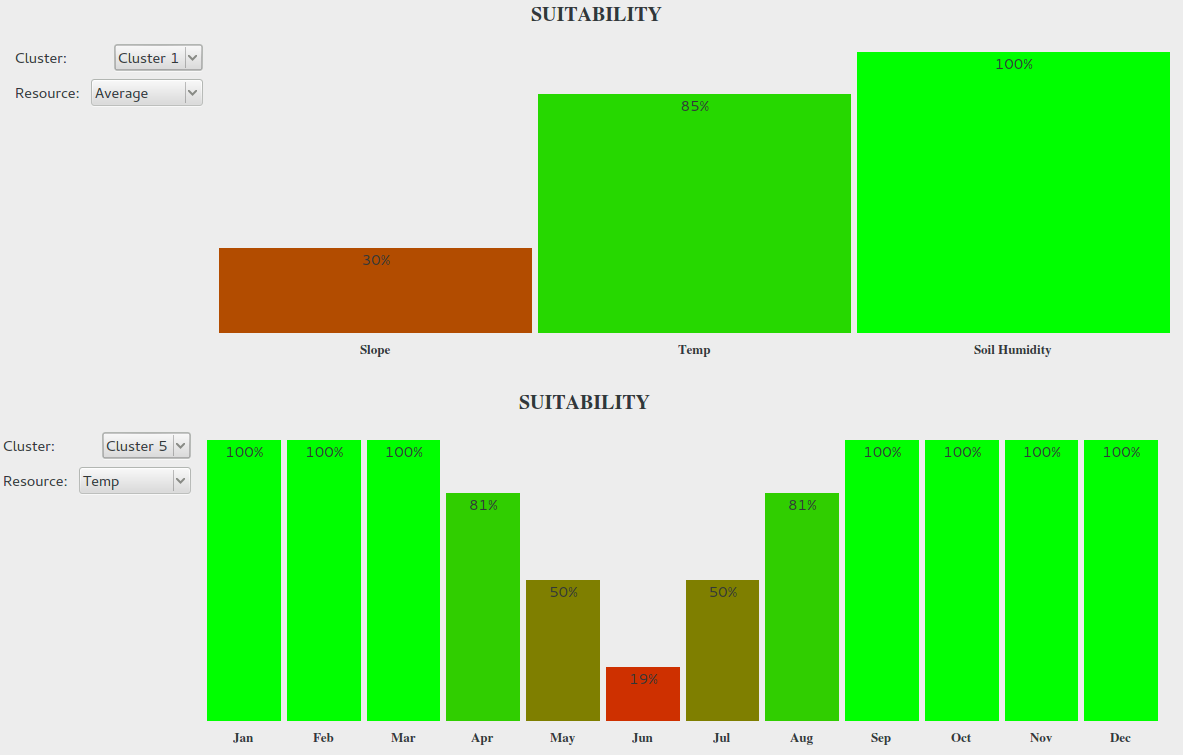
\includegraphics[width=\textwidth]{specie_suitability_temp_and_avg.png}
	\caption{ Overall (top) and temperature (bottom) intermediate species suitability histograms. Not displayed but also generated are the illumination and humidity intermediate species suitability histograms.}	
	\label{fig:specie_intermediate_suitability_scores}
\end{figure}


